Finally, I want to take a closer look at a more recently developed architecture called EfficientNet. Its name indicates its goal, being more efficient than previous attempts. To achieve this, \citet{tan2020efficientnet} tried different scaling methods on a conventional deep network. 

\begin{figure}[h]
\centering
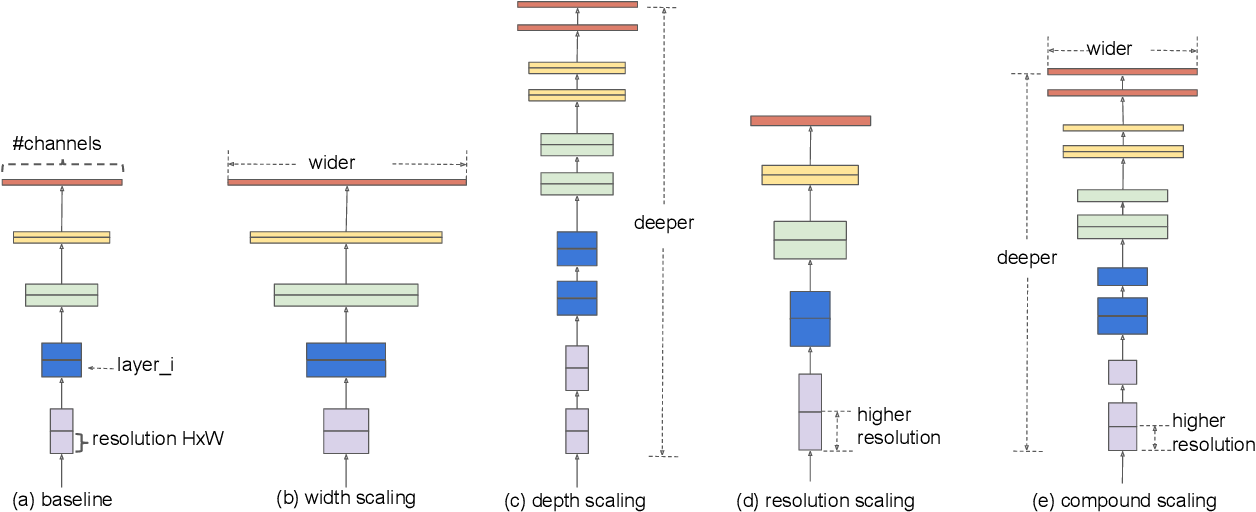
\includegraphics[width=\textwidth]{images/Chapter2/2-Figure2-1 (1).png}
\caption{Different scaling approaches for improving efficiency by keeping (or ideally improving) accuracy for deep learning architectures \citep{tan2020efficientnet}. } 
\label{fig:effnet_scaling}
\end{figure}

They chose three parameters to vary and optimize efficiency and accuracy along the way: the input resolution, the number of layers and the number of channels of each output. The latter is called width scaling, increasing the number of layers is depth scaling and changing the resolution is resolution scaling. A change of all parameters is referred to as compound scaling. They developed a neural network based on the approach by \citet{tan2019mnasnet} with a cost function that optimizes the amount of \textit{floating point operations per second} (FLOPS) by keeping a set accuracy, allowing them to develop a set of CNNs that achieve high accuracies with less operations and parameters needed in training. EfficientNet-B7, which I will use in training, has 66 million parameters, only six million more than the 60 million of ResNet152 by being significantly more accurate (see \autoref{fig:effnet_params}). \\
This indicates that the future of image recognition and classification won't be developed by humans alone, but by algorithms searching for the best model for a certain task.

\begin{figure}[H]
\centering
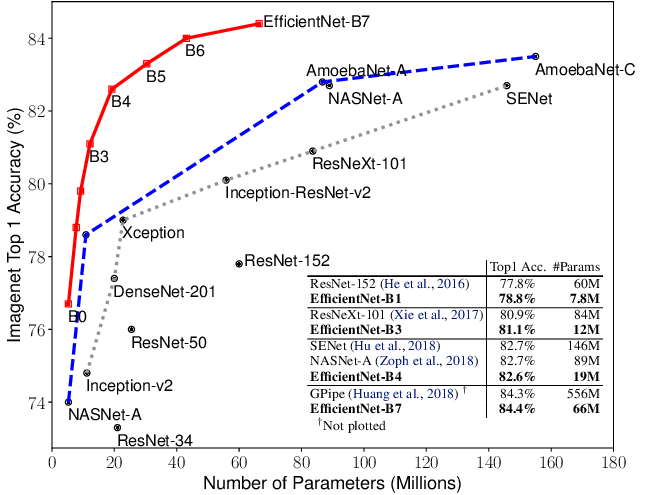
\includegraphics[width=.5\textwidth]{images/Chapter2/1-Figure1-1.png}
\caption{Comparison between the accuracy and number of parameters of EfficientNets and other successful CNN models \citep{tan2020efficientnet}. } 
\label{fig:effnet_params}
\end{figure}

After this brief introduction to the architectures used in my thesis, I want to talk about the implementation of them and the data that they will be provided with in training. 
